\section{Systemübersicht}
\subsection{Grobe Systemübersicht}
Es soll eine bereits bestehende Java Game-Applikation mit einem voll funktionalen Logger erweitert werden. Dieser soll die Log-Einträge auf der Applikation-Seite entgegennehmen und danach über TCP/IP jene Events an einen Server senden. Der Server soll all diese Pakete entgegennehmen und in einem vordefinierten Format in eine dafür definierte Datei schreiben. 
Das System soll folgendermassen dargestellt werden:
\begin{figure}[H]
	\centering
	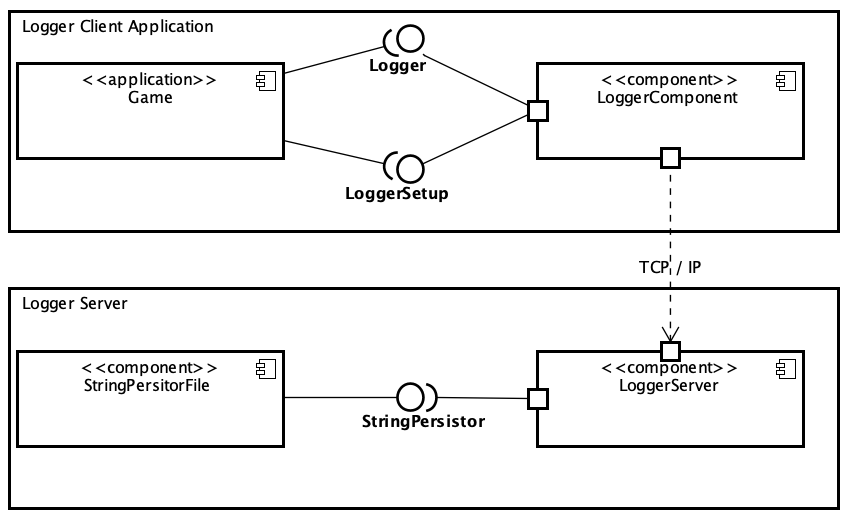
\includegraphics[width=\textwidth]{1_Systemuebersicht/Bilder/componentDiagram.png}
	\caption{Komponentendiagram}
	\label{fig:Komponentendiagramm}
\end{figure}